\chapter{Introducción específica} % Main chapter title

\label{Chapter2}

%----------------------------------------------------------------------------------------
%	Chapter 2
%----------------------------------------------------------------------------------------

Este capítulo lista los requerimientos y en base a ellos presenta y describe los componentes internos del sistema desarrollado, junto con las tecnologías y recursos de software utilizados para su implementación. Asimismo se realiza una descripción simplificada del funcionamiento de un EDFA.

\section{Requerimientos}

Los requerimientos fueron determinados en conjunto con la empresa en base a las funcionalidades y prestaciones con las que debe contar el sistema. Como la lista es muy extensa, se listan a continuación solamente algunos de los principales:

\renewcommand{\labelenumii}{\arabic{enumi}.\arabic{enumii}}

\begin{enumerate}

\item Encendido y apagado del EDFA
	\begin{enumerate}
	\item El software debe apagar la salida óptica del dispositivo 			EDFA bajo prueba cuando se detecte la activación de alguna de las 		alarmas.
	\item Mediante la función táctil de la pantalla LCD el usuario 			debe poder prender y apagar la alimentación del dispositivo EDFA 		bajo prueba y su salida óptica.
	\item El software debe cortar la alimentación del dispositivo EDFA 	bajo prueba cuando se detecte que la corriente supera el valor 			previamente definido.
	\item El software debe medir y mostrar en pantalla los valores de 		tensión de alimentación y consumo de corriente del dispositivo 			EDFA bajo prueba mediante las señales analógicas de entrada 			provenientes de los respectivos monitores, con una precisión no 		menor al 10\% (máximo desvío con respecto al valor real). Este 			valor debe ser de una cifra significativa para la parte entera y 		dos para la decimal.
	\end{enumerate}

\item Pantalla LCD
	\begin{enumerate}
	\item El software debe actualizar la imagen de la pantalla cada 		medio segundo (2 cuadros por segundo).
	\item La pantalla deberá indicar el estado de la salida óptica del 	dispositivo EDFA bajo prueba y el del relé de alimentación.
	\item Mediante la función táctil de la pantalla LCD el usuario 			debe poder cambiar el valor para el cual se detecta una 				sobrecorriente. El rango válido para este valor debe ser de 0 A a 		3 A, siendo la parte decimal de dos cifras significativas.
	\end{enumerate}
	
\item Entradas y salidas del EDFA
	\begin{enumerate}
	\item El software deberá mostrar en la pantalla los estados de todas las señales digitales de entrada y salida del dispositivo EDFA bajo prueba.
	\end{enumerate}

\item Requisitos de rendimiento
	\begin{enumerate}
	\item La apertura del relé de alimentación del dispositivo EDFA 		bajo prueba deberá efectuarse en un tiempo menor a 50 ms luego de 		detectarse una sobrecorriente o una caída de la tensión de 				alimentación.
	\item El apagado de la salida óptica del dispositivo EDFA bajo 			prueba deberá efectuarse en un tiempo menor a 100 ms luego de 			detectarse la activación de una alarma.
	\end{enumerate}
	
\end{enumerate}

La lista completa de requerimientos se puede ver en \citep{DOC_REQ}.

\section{Funcionamiento de un amplificador óptico}
\label{sec:funcAmp}

Los amplificadores de fibra dopados con erbio son los amplificadores ópticos más importantes en el contexto de comunicaciones ópticas de larga distancia. Son utilizados en la banda L y C del espectro (aproximadamente entre 1550 nm y 1650 nm), región en la que las pérdidas en la fibra óptica son menores. Esto se puede ver en la figura \ref{fig:espectro}, que muestra las pérdidas en función de la longitud de onda de la luz utilizada.

\begin{figure}[H]
\centering
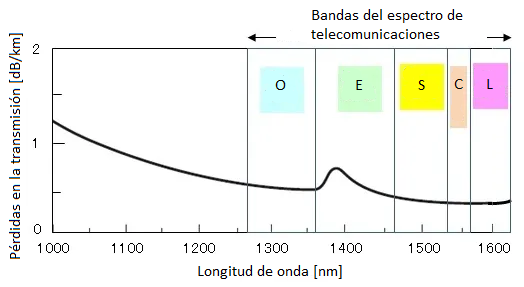
\includegraphics[width=0.85\textwidth]{./Figures/espectro.png}
\caption{Pérdidas en la fibra.}
\label{fig:espectro}
\end{figure}

Inventado en 1987, el EDFA es generalmente usado para compensar las pérdidas mencionadas en una línea de transmisión óptica. Éste puede ser colocado en tres partes: 

\begin{itemize}
\item Inmediatamente después del transmisor, para aumentar la potencia inyectada en la línea
\item En el medio del camino óptico, para compensar las pérdidas por la distancia recorrida
\item Antes del receptor, para favorecer la detección de la señal
\end{itemize}

La figura \ref{fig:EDFAinterno} muestra la configuración interna más común de un EDFA. Su componente principal es la fibra dopada con erbio (EDF por sus siglas en inglés), que generalmente es monomodo\protect\footnotemark . 

\footnotetext{Tipo de fibra óptica en la que solo se propaga un modo de luz, paralela al eje de la fibra. Tienen un tamaño entre 8.3 y 10 micrones, permiten alcanzar distancias de hasta 400 km y tasas de transmisión de hasta 10 Gbps \citep{WEBSITE:FIBRA}.}

La luz ingresa al amplificador mediante el puerto de entrada y luego mediante un divisor se redirige un porcentaje de la señal (generalmente entre un 1\% y 2\%) a un detector para realizar una medición de la potencia óptica. Luego, pasa por un aislador óptico que permite la transmisión de luz en un solo sentido y así evita una realimentación debida a reflexiones en etapas posteriores.

La bomba de 980 nm es un diodo láser que genera una señal que se combina con la señal entrante (ahora a la salida del aislador) y pasan por la fibra dopada con erbio. En esta instancia es donde se genera la amplificación de la señal propiamente dicha, mediante un efecto denominado emisión estimulada\protect\footnotemark .

\footnotetext{Proceso por el cual un fotón incidente de una determinada frecuencia interactúa con un electrón excitado, causando que éste caiga a un nivel de energía menor. La energía liberada se transfiere al campo electromagnético, creando un nuevo fotón con la misma frecuencia, polarización y dirección de movimiento que el fotón incidente \citep{WEBSITE:EMISSION}.}

\begin{figure}[H]
\centering
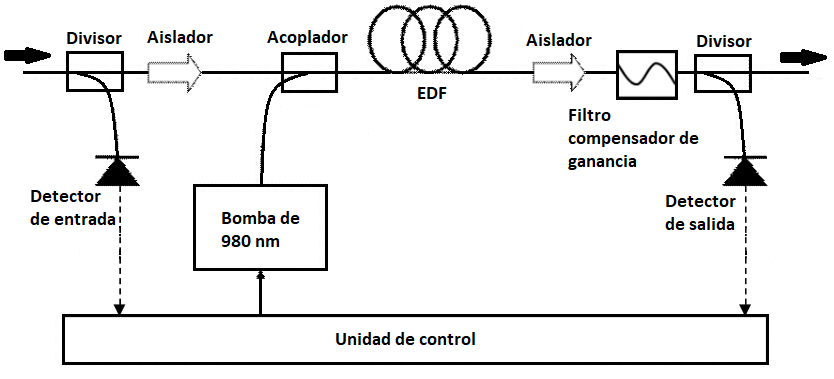
\includegraphics[width=0.85\textwidth]{./Figures/EDFAinterno.png}
\caption{Configuración interna de un EDFA.}
\label{fig:EDFAinterno}
\end{figure}

Una vez amplificada, la señal pasa nuevamente por otro aislador que se encarga principalmente de filtrar la luz de 980 nm, evitando que se introduzca en el camino óptico. Luego, la señal pasa por un filtro compensador de ganancia (GFF por sus siglas en inglés) cuyo objetivo es hacer constante la ganancia del amplificador en todo el ancho de banda de trabajo (bandas C y L del espectro). Finalmente, antes de que la luz salga del amplificador, se realiza nuevamente una medición de la potencia óptica al igual que en la entrada.

Tanto la bomba de 980 nm como ambos detectores de potencia se encuentran conectados a una unidad de control. Ésta generalmente cuenta con un microcontrolador o chip dedicado que se encarga de regular la potencia que entrega la bomba en base a los valores medidos por los detectores, creando un lazo de control automático de ganancia \citep{WEBSITE:EDFA1}\citep{WEBSITE:EDFA2}.

\section{Interfaz del amplificador óptico}
\label{sec:intAmp}

Como se mencionó en la sección \ref{sec:contexto}, para poder controlarlo, el EDFA cuenta con un conector de 25 pines tipo microD. Este conector contiene varios grupos de señales con distintas funciones. La tabla \ref{tab:señalesConector} lista cada una de las señales de la interfaz, junto con los detalles de su dirección, tipo y función.

\begin{table}[H]
	\centering
	\caption{Señales de la interfaz del EDFA.}
	\begin{tabular}{l c p{1.5cm} p{5cm}}
		\toprule
		\textbf{Nombre de la señal}	& \textbf{Dirección}	& \textbf{Tipo} & \textbf{Función} \\
		\midrule
		5V 					& Entrada	& Potencia			& Entrada de alimentación del EDFA \\		
		PGND				& Salida	& Potencia  		& Retorno de alimentación (potencia) \\
		GND					& Salida	& Tierra digital  	& Retorno de alimentación (digital) \\
		IN\_POW				& Salida	& Analógica 		& Indica el nivel de potencia óptica de entrada \\
		OUT\_POW			& Salida	& Analógica 		& Indica el nivel de potencia óptica de salida \\
		CASE\_TEMP\_ALARM	& Salida	& Digital 			& Alarma de temperatura de la carcasa del EDFA \\
		PUMP\_BIAS\_ALARM	& Salida	& Digital 			& Alarma de la bomba de polarización \\
		OUT\_POW\_ALARM		& Salida	& Digital 			& Alarma de nivel de potencia de salida \\
		IN\_POW\_ALARM		& Salida	& Digital 			& Alarma de nivel de potencia de entrada \\
		EN/DIS				& Entrada	& Digital 			& Habilitación del amplificador \\
		RESET\_uC			& Entrada	& Digital 			& Reset del microcontrolador del EDFA \\
		OUT\_POW\_MUTE		& Entrada	& Digital 			& Habilitación de la salida óptica \\
		UART\_TX			& Salida	& Digital 			& Transmisor del UART interno del EDFA \\
		UART\_RX			& Entrada	& Digital 			& Receptor del UART interno del EDFA \\
		\bottomrule
		\hline
	\end{tabular}
	\label{tab:señalesConector}
\end{table}

A continuación, se provee una breve explicación de cada grupo de señales:
\begin{itemize}
\item Alimentación: tiene separada la tierra en digital, para la lógica y la comunicación, y la de potencia para la amplificación de la señal óptica
\item Señales analógicas: indican el nivel de potencia óptica de entrada y salida del EDFA
\item Alarmas: Mediante un estado en alto indican si ocurrió alguno de los eventos que requieren la atención del usuario
\item Señales de control: Controlan el funcionamiento de ciertos componentes del amplificador
\item Comunicación UART: Permite el envío de comandos al EDFA y la consulta de valores de parámetros internos como temperaturas, potencias, ganancias, etc.
\end{itemize}

\section{Componentes del sistema}

Los componentes de hardware que forman parte del sistema presentado en la sección \ref{sec:contexto} fueron seleccionados con el objetivo de cumplir con los requisitos y a su vez utilizar la menor cantidad posible. Así se logra mantener al sistema simple, con poca probabilidad de fallas, fácil de usar y probar. A continuación se presentan los principales componentes y sus características.

\subsection{Microcontrolador}

El modelo de microcontrolador utilizado es el STM32F429, del fabricante ST y con arquitectura de procesador ARM Cortex-M.

La principal razón por la que se decidió utilizar este modelo es porque es el que se encuentra integrado en la placa de desarrollo Nucleo-144, utilizada durante la cursada de la Especialización. Algunas de sus características más relevantes para esta aplicación son \citep{STM32F429}:

\begin{itemize}
\item Núcleo CPU Arm® Cortex®-M4 de 32 bits con unidad de punto flotante, frecuencia hasta 180 MHz, unidad de protección de memoria e instrucciones DSP
\item Memoria Flash de hasta 2 MB
\item Interfaces de comunicación:
	\begin{itemize}
	\item 3 interfaces I2C
	\item 4 UART/USART (hasta 11.25 Mbit/s)
	\item 6 interfaces SPI (hasta 45 Mbit/s)
	\end{itemize}
\item Hasta 168 puertos de entrada/salida con interrupción
\item 3 conversores ADC de 12 bit de resolución y 2.4 MSPS. Hasta 24 canales
\item DMA de propósito general con FIFO y soporte de ráfaga
\item Interfaces SWD y JTAG para depuración
\item Hasta 12 \textit{timers} de 16 bits con IC/OC y PWM
\end{itemize}

La alta velocidad de reloj, la gran capacidad de memoria Flash y la gran cantidad de periféricos disponibles hacen a este modelo ideal para la ejecución de un RTOS.

La principal ventaja de utilizar la placa de desarrollo Nucleo-144 es que esta ya trae incorporada la interfaz de programación y depuración ST-LINK/V2 \citep{NUCLEO144}.

\subsection{Monitor de corriente}

El circuito integrado elegido para efectuar la medición de corriente de alimentación del amplificador mientras este se encuentra en funcionamiento es el INA301A3. Sus principales características son:

\begin{itemize}
\item Alto rango de tensión de modo común (0 V a 36 V)
\item Salida analógica y a comparador
\item Máxima tensión de \textit{offset} de salida: 35 uV
\item Máximo error de ganancia: 0.1%
\item Ganancia del amplificador: 100 V/V
\item Nivel de alerta programable mediante un resistor
\item Tiempo total de respuesta de la alerta: 1 us
\end{itemize}

Este chip provee en uno de sus pines una tensión analógica proporcional a la corriente que se está midiendo. Asimismo, cuenta con una salida digital que se activa cuando la corriente medida alcanza cierto nivel establecido mediante un resistor (pin ALERT) \citep{INA301}.

\subsection{Pantalla táctil LCD}
\label{sec:pantLCD}

El modelo del módulo de la pantalla LCD utilizada en el trabajo es MSP2807, que es una solución integrada, es decir, cuenta con toda la electrónica necesaria para poder hacer uso de la pantalla en su totalidad. Para esto cuenta con dos circuitos integrados: el controlador del display de la pantalla (lo que permite dibujar en ella) y el controlador de la función táctil (lo que permite detectar cuando se la toca). En la figura \ref{fig:pantLCD} se puede ver una imagen de la pantalla.

\begin{figure}[H]
\centering
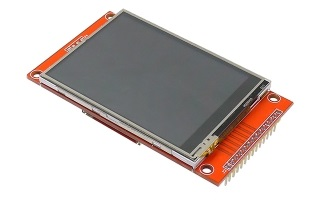
\includegraphics[width=0.7\textwidth]{./Figures/pant_LCD.png}
\caption{Pantalla LCD táctil MSP2807.}
\label{fig:pantLCD}
\end{figure}

En la tabla \ref{tab:caractLCD} se listan las características de la pantalla.

\begin{table}[H]
	\centering
	\caption{Características de la pantalla LCD.}
	\begin{tabular}{l c}
		\toprule
		\textbf{Característica}	& \textbf{Valor} \\
		\midrule
		Color				& 65K colores RGB \\
		Tamaño				& 2.8 pulgadas (7.11 cm) \\
		Tipo de pantalla	& TFT \\
		Resolución			& 320x240 pixeles \\
		Área activa			& 43.2x57.6 mm \\
		Tensión de alimentación		& 3.3 V - 5 V \\
		Nivel lógico de I/O			& 3.3 V (TTL) \\		
		\bottomrule
		\hline
	\end{tabular}
	\label{tab:caractLCD}
\end{table}

El controlador del display tiene una interfaz SPI para el envío de los datos y además una señal denominada DC/RS para indicar si lo que está enviando el maestro es un dato o un registro interno del chip. También consta de una señal de reset para borrar todo el contenido del display.

El controlador de la función táctil también tiene un bus SPI y una señal adicional de interrupción denominada T\_IRQ que indica cuando el display está siendo tocado \citep{MSP2807}.

\section{Recursos de software}

Para el firmware del microcontrolador se usaron distintas herramientas que permitieron el desarrollo de una estructura de software jerárquica, simple y eficaz.

\subsection{Sistema operativo de tiempo real FreeRTOS}

FreeRTOS es un sistema operativo de tiempo real o RTOS (de \textit{Real Time Operating System}) para microcontroladores o pequeños microprocesadores, diseñado para ocupar poco espacio, ser confiable y fácil de usar. Está escrito en C para que sea fácil de mantener y trasladar a nuevos dispositivos.

FreeRTOS provee recursos que facilitan la ejecución de aplicaciones sobre el sistema operativo como tareas, semáforos, \textit{mutexes}, temporizadores por software, colas y gestores de memoria dinámica \citep{WEBSITE:1}.

Si se separa el firmware en capas desde la más baja (hardware) hasta la más alta (aplicación de usuario) el lugar que ocupa FreeRTOS se ubica por arriba de los drivers provistos por el fabricante, brindando una capa de abstracción de mayor nivel. De esta forma, el sistema operativo actúa como puente entre las capas más bajas y las más altas, gestionando los recursos de hardware de forma automática y brindando servicios a la capa de aplicación.

En la figura \ref{fig:capas} se puede ver la estructura de capas del firmware con FreeRTOS incluida.

\begin{figure}[H]
\centering
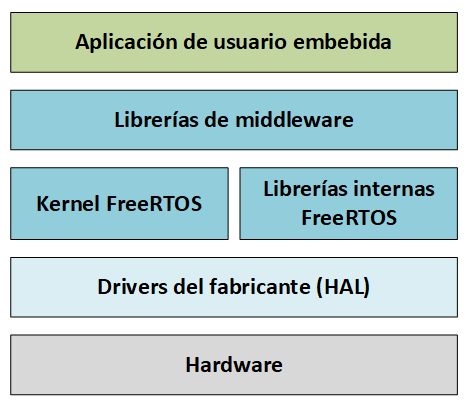
\includegraphics[width=0.65\textwidth]{./Figures/capas.png}
\caption{Estructura de capas con FreeRTOS.}
\label{fig:capas}
\end{figure}

Uno de las ventajas principales de usar FreeRTOS es la posibilidad de ejecutar varias tareas o \textit{tasks} en forma simultánea tal como lo hace un sistema operativo cualquiera. Un \textit{scheduler} gestiona la ejecución de cada una de forma individual y con su propio contexto (\textit{stack} y variables). Esto permite estructurar la aplicación separándola en tareas independientes pero sincronizadas \citep{WEBSITE:FREERTOS}.

\subsection{Capa de abstracción de hardware (HAL)}

Una \textit{hardware abstraction layer} o HAL es un conjunto de rutinas de software que brinda acceso a recursos de hardware a programas de aplicación. Se ubica inmediatamente por arriba del hardware y por debajo del sistema operativo que se ejecuta, como se puede ver en la figura \ref{fig:capas}.

La principal ventaja de esta capa es que oculta la arquitectura del hardware del \textit{kernel} del sistema operativo. Así, el código del \textit{kernel} no tiene que ser cambiado o reescrito para que pueda correr sobre sistemas con distinto hardware y las aplicaciones de software se vuelven independientes de la plataforma (portabilidad) \citep{WEBSITE:HAL}.

La HAL de la serie de microcontroladores STM32 se denomina STM32Cube y tiene como objetivo asegurar la máxima portabilidad entre dispositivos de la misma familia y proveer APIs (\textit{Application Programming Interface}) multi-instancia para todos los periféricos (UART, SPI, temporizadores, ADC, etc.). Éstas APIs están listas para usar y facilitan la implementación de la aplicación de usuario. Por ejemplo, los periféricos de comunicación cuentan con APIs para inicializarlos y configurarlos, gestionar la transferencia de datos en modo \textit{polling}, manejar las interrupciones, el DMA (\textit{Direct Memory Access}) y los errores de comunicación \citep{WEBSITE:STM32CUBE}.

\section{Periféricos utilizados}

A excepción del monitor de corriente, el resto de los periféricos utilizados ya se encuentran integrados en el chip del microcontrolador, por lo que no hubo que agregar ningún hardware adicional y para poder utilizarlos solo hizo falta leer las hojas de datos. De todas formas, en esta sección se provee una breve descripción de cada uno.

\subsection{Conversor analógico-digital (ADC)}

Un conversor analógico-digital o ADC (de \textit{Analog-to-Digital Converter}) es un dispositivo que convierte una señal eléctrica analógica proveniente, por ejemplo, de un sensor a una señal digital. La principal ventaja de esta conversión es que su valor puede ser almacenado en un sistema digital, por lo que estará representada por un número binario.

La señal pasa de ser continua en el tiempo y continua en amplitud a discreta en el tiempo y discreta en amplitud. Esto quiere decir que la señal analógica podría tomar cualquier valor en cualquier instante. En cambio, cuando es convertida la señal se encuentra cuantizada, es decir, podrá tomar solamente determinados valores que dependen de la cantidad de bits del ADC y del fondo de escala (resolución).

Esto hace que no se puedan representar todos los valores que se miden y que cada muestra tomada estará truncada al valor más cercano representable. Este error introducido en la medición se denomina error de cuantización. A modo de ejemplo, en la figura \ref{fig:muestreoADC} se muestra una conversión analógica-digital de una señal senoidal con un ADC de 3 bits. La señal de entrada (en rojo) es muestreada a intervalos constantes y la señal resultante (en azul) está cuantizada.

\begin{figure}[H]
\centering
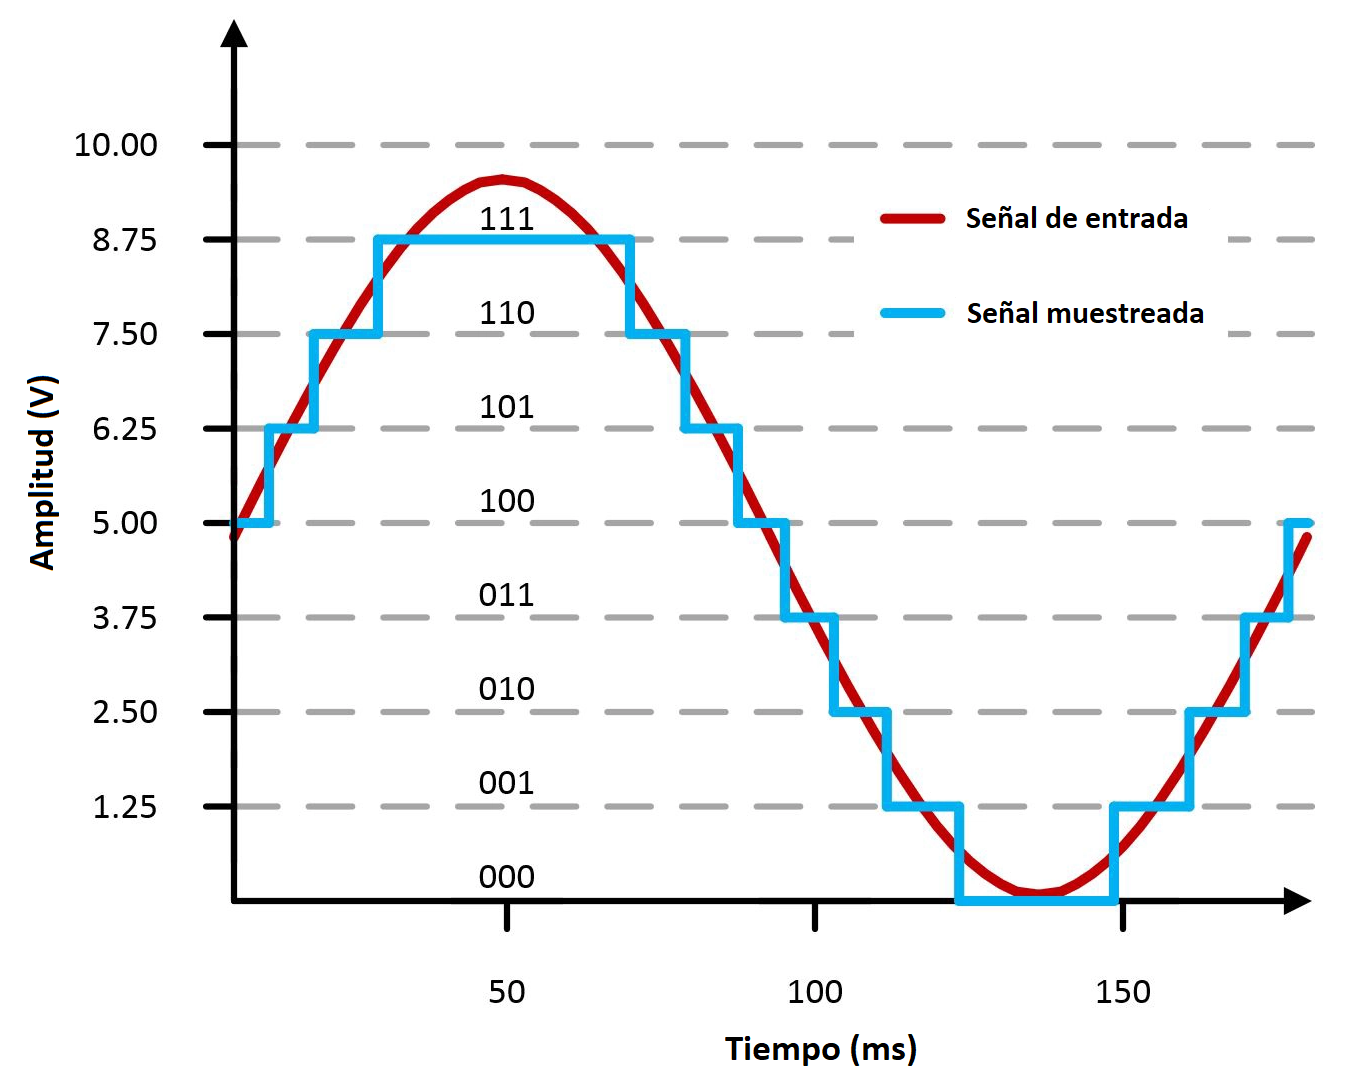
\includegraphics[width=0.65\textwidth]{./Figures/muestreo.png}
\caption{Conversión de una señal con un ADC de 3 bits.}
\label{fig:muestreoADC}
\end{figure}

De la figura \ref{fig:muestreoADC} se ve que mientras más bits de resolución tenga el ADC, se pueden tomar valores más cercanos al medido y por lo tanto tener una mejor representación de la señal.

Esto impacta directamente en el parámetro de relación señal-ruido que, junto con el ancho de banda (velocidad de muestreo), es uno de los parámetros con los que se caracteriza el rendimiento de un ADC \citep{WEBSITE:2}.

\subsection{Universal Asynchronous Receiver Transmitter (UART)}

Un UART es un dispositivo utilizado para establecer una comunicación serie asíncrona, con formato de datos y velocidad de transmisión configurables. Consta solo de dos señales que conectan dos dispositivos de forma bidireccional: una para la transmisión y otra para la recepción, comúnmente llamadas TX y RX respectivamente.

La forma de transmisión de datos del protocolo tiene una estructura fija. Por cada dato que se transmite (cuyo ancho puede variar entre 5 y 9 bits), se transmiten además bits adicionales de comienzo y fin de trama (\textit{Start} y \textit{Stop}) y, opcionalmente, los de paridad para la detección de errores. En la figura \ref{fig:transUART} se puede ver la composición de una trama completa.

\begin{figure}[H]
\centering
\includegraphics[width=0.9\textwidth]{./Figures/UART_frame.png}
\caption{Trama de transmisión UART.}
\label{fig:transUART}
\end{figure}

Los bits de \textit{Start} y \textit{Stop} son para indicarle al receptor cuando debe comenzar y cuando parar de tomar los datos transmitidos. También sirve para realizar una sincronización de los relojes del transmisor y del receptor. Como el protocolo es asíncrono, es decir, no transmite el reloj en ninguna de sus líneas, los relojes internos de ambos deben estar en fase.

El estado \textit{Idle} de la línea es el estado inactivo, es decir, el estado de reposo cuando no se encuentra transmitiendo \citep{WEBSITE:3}.

\subsection{Serial Peripheral Interface (SPI)}

SPI es una especificación de interfaz de comunicación serie sincrónica para distancias cortas. Es comúnmente utilizada para enviar datos entre un sistema embebido y pequeños periféricos como sensores y memorias SD.

Los dispositivos SPI se comunican en modo \textit{full duplex} (ambos sentidos simultáneos) mediante una arquitectura maestro-esclavo con líneas separadas para los datos y el clock. Generalmente constan de 4 líneas:

\begin{itemize}
\item SCLK: reloj o clock (generado por el maestro)
\item MOSI: \textit{Master Out Slave In}. Salida de datos de maestro a esclavo
\item MISO: \textit{Master In Slave Out}. Salida de datos de esclavo a maestro
\item CS/SS: \textit{Chip Select}. Salida de maestro para indicar al esclavo que se están enviando o recibiendo datos
\end{itemize}

Para comenzar la comunicación el maestro primero configura el clock, utilizando una frecuencia soportada por el dispositivo esclavo, generalmente entre 100 kHz y 10 MHz. Luego selecciona el esclavo poniendo un nivel bajo en la línea CS. En este momento, a veces, se requiere un tiempo mínimo de espera antes de enviar ciclos de clock, por ejemplo para una conversión analógico-digital.

Durante cada ciclo de clock ocurre una transmisión \textit{full duplex}. El maestro envía un bit por la línea MOSI y el esclavo la lee, mientras que el esclavo envía otro bit por la línea MISO y el maestro la lee. Ésta secuencia se mantiene incluso cuando se está enviando un dato en una sola dirección.

En la figura \ref{fig:transSPI} se pueden ver las señales durante una transacción de maestro a esclavo y de esclavo a maestro. Se observa que la señal CS se mantiene en nivel bajo durante todo el tiempo en que la transmisión está activa. Además, las transiciones de las señales MOSI y MISO para cada bit ocurren solamente en cada flanco negativo del clock. En este caso el ancho de la palabra transmitida es de 8 bits, pero se puede implementar de igual forma para cantidades mayores o menores. Esto es posible debido a que no existe un protocolo estándar para la transmisión SPI.

\begin{figure}[H]
\centering
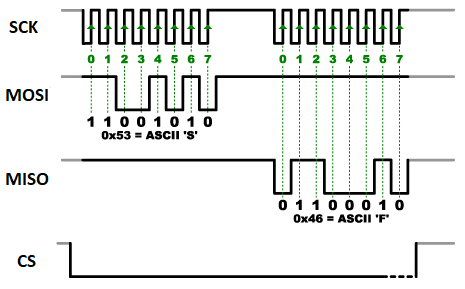
\includegraphics[width=0.85\textwidth]{./Figures/SPItrans.png}
\caption{Transacción SPI.}
\label{fig:transSPI}
\end{figure}

En el caso de la figura \ref{fig:transSPI} el nivel del clock cuando la interfaz se encuentra inactiva (\textit{Idle}) es alto y el flanco en que cambia el bit transmitido es descendente pero, al igual que la velocidad de transmisión, estos parámetros pueden ser configurados con distintos valores por el maestro antes de realizar cada transacción.

El hecho de contar con una línea de selección de esclavo permite realizar una conexión de un maestro con múltiples esclavos simplemente agregando una línea CS por cada esclavo y reutilizando las demás, como se observa en la figura \ref{fig:multiSlave}. De esta forma, si un esclavo recibe ciclos de clock y datos pero no está habilitado mediante la señal CS, los descartará \citep{WEBSITE:SPI}.

\begin{figure}[H]
\centering
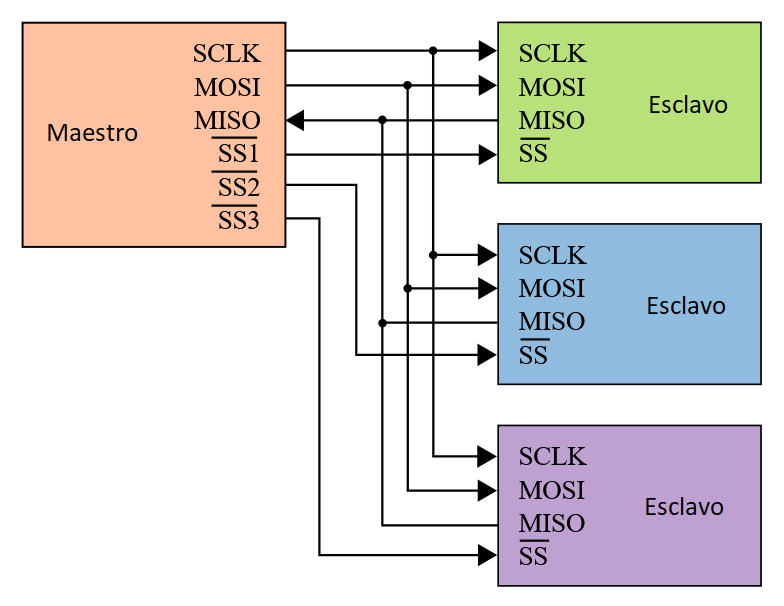
\includegraphics[width=0.65\textwidth]{./Figures/multiSlave.png}
\caption{Conexionado de un maestro con múltiples esclavos.}
\label{fig:multiSlave}
\end{figure}

A diferencia de otros protocolos como UART, SPI define solamente una estructura de hardware para la transmisión de información. No define un protocolo para los datos transmitidos. Esto quiere decir que los bits transmitidos no tienen una función determinada predefinida si no que ésta es específica de la aplicación y corre por parte del hardware (o software) realizar la interpretación correcta.
